\documentclass[twoside]{book}

% Packages required by doxygen
\usepackage{fixltx2e}
\usepackage{calc}
\usepackage{doxygen}
\usepackage[export]{adjustbox} % also loads graphicx
\usepackage{graphicx}
\usepackage[utf8]{inputenc}
\usepackage{makeidx}
\usepackage{multicol}
\usepackage{multirow}
\PassOptionsToPackage{warn}{textcomp}
\usepackage{textcomp}
\usepackage[nointegrals]{wasysym}
\usepackage[table]{xcolor}

% Font selection
\usepackage[T1]{fontenc}
\usepackage[scaled=.90]{helvet}
\usepackage{courier}
\usepackage{amssymb}
\usepackage{sectsty}
\renewcommand{\familydefault}{\sfdefault}
\allsectionsfont{%
  \fontseries{bc}\selectfont%
  \color{darkgray}%
}
\renewcommand{\DoxyLabelFont}{%
  \fontseries{bc}\selectfont%
  \color{darkgray}%
}
\newcommand{\+}{\discretionary{\mbox{\scriptsize$\hookleftarrow$}}{}{}}

% Page & text layout
\usepackage{geometry}
\geometry{%
  a4paper,%
  top=2.5cm,%
  bottom=2.5cm,%
  left=2.5cm,%
  right=2.5cm%
}
\tolerance=750
\hfuzz=15pt
\hbadness=750
\setlength{\emergencystretch}{15pt}
\setlength{\parindent}{0cm}
\setlength{\parskip}{0.2cm}
\makeatletter
\renewcommand{\paragraph}{%
  \@startsection{paragraph}{4}{0ex}{-1.0ex}{1.0ex}{%
    \normalfont\normalsize\bfseries\SS@parafont%
  }%
}
\renewcommand{\subparagraph}{%
  \@startsection{subparagraph}{5}{0ex}{-1.0ex}{1.0ex}{%
    \normalfont\normalsize\bfseries\SS@subparafont%
  }%
}
\makeatother

% Headers & footers
\usepackage{fancyhdr}
\pagestyle{fancyplain}
\fancyhead[LE]{\fancyplain{}{\bfseries\thepage}}
\fancyhead[CE]{\fancyplain{}{}}
\fancyhead[RE]{\fancyplain{}{\bfseries\leftmark}}
\fancyhead[LO]{\fancyplain{}{\bfseries\rightmark}}
\fancyhead[CO]{\fancyplain{}{}}
\fancyhead[RO]{\fancyplain{}{\bfseries\thepage}}
\fancyfoot[LE]{\fancyplain{}{}}
\fancyfoot[CE]{\fancyplain{}{}}
\fancyfoot[RE]{\fancyplain{}{\bfseries\scriptsize Generated on Fri Jan 2 2015 18\+:01\+:40 for C\+L\+Utils by Doxygen }}
\fancyfoot[LO]{\fancyplain{}{\bfseries\scriptsize Generated on Fri Jan 2 2015 18\+:01\+:40 for C\+L\+Utils by Doxygen }}
\fancyfoot[CO]{\fancyplain{}{}}
\fancyfoot[RO]{\fancyplain{}{}}
\renewcommand{\footrulewidth}{0.4pt}
\renewcommand{\chaptermark}[1]{%
  \markboth{#1}{}%
}
\renewcommand{\sectionmark}[1]{%
  \markright{\thesection\ #1}%
}

% Indices & bibliography
\usepackage{natbib}
\usepackage[titles]{tocloft}
\setcounter{tocdepth}{3}
\setcounter{secnumdepth}{5}
\makeindex

% Hyperlinks (required, but should be loaded last)
\usepackage{ifpdf}
\ifpdf
  \usepackage[pdftex,pagebackref=true]{hyperref}
\else
  \usepackage[ps2pdf,pagebackref=true]{hyperref}
\fi
\hypersetup{%
  colorlinks=true,%
  linkcolor=blue,%
  citecolor=blue,%
  unicode%
}

% Custom commands
\newcommand{\clearemptydoublepage}{%
  \newpage{\pagestyle{empty}\cleardoublepage}%
}


%===== C O N T E N T S =====

\begin{document}

% Titlepage & ToC
\hypersetup{pageanchor=false,
             bookmarks=true,
             bookmarksnumbered=true,
             pdfencoding=unicode
            }
\pagenumbering{roman}
\begin{titlepage}
\vspace*{7cm}
\begin{center}%
{\Large C\+L\+Utils \\[1ex]\large 0.\+1 }\\
\vspace*{1cm}
{\large Generated by Doxygen 1.8.9}\\
\vspace*{0.5cm}
{\small Fri Jan 2 2015 18:01:40}\\
\end{center}
\end{titlepage}
\clearemptydoublepage
\tableofcontents
\clearemptydoublepage
\pagenumbering{arabic}
\hypersetup{pageanchor=true}

%--- Begin generated contents ---
\chapter{C\+L\+Utils Documentation}
\label{index}\hypertarget{index}{}\section*{C\+L\+Utils }

C\+L\+Utils offers utilities that help setup and manage an Open\+C\+L environment. It aims to allow rapid prototyping by hiding away all the boilerplate code necessary for establishing an Open\+C\+L environment.

This meant to be an exercise on how I would go about containing the Open\+C\+L objects, and developing an A\+P\+I to interface them all. But since I didn\textquotesingle{}t have a solid idea of what I needed, I started writing the code and ended up adapting the A\+P\+I around it. The result was an A\+P\+I that made use of indices to refer to Open\+C\+L objects which only makes it efficient to use under a known environment. Nonetheless, the library works pretty robustly. Now that I have a better understanding on the problem, I intent to come back at some point and reconfigure the whole thing.

If you would like something more appropriate and complete, take a look at \href{https://github.com/kylelutz/compute}{\tt boost.\+compute} or \href{http://developer.amd.com/tools-and-sdks/opencl-zone/amd-accelerated-parallel-processing-app-sdk/}{\tt A\+M\+D A\+P\+P S\+D\+K\textquotesingle{}s C\+L\+Util}.

~\newline
 \section*{A\+P\+I }



~\newline
~\newline
 The simplest case covered by the library is one where a context is created for the first platform returned by the Open\+C\+L A\+P\+I, and a command queue is created for the first device in that platform. Programs are built for all devices in the associated context. This case is covered automatically when a kernel filename is provided on the definition of a {\ttfamily C\+L\+Env} instance.

\begin{quote}
\#include $<$\hyperlink{CLUtils_8hpp}{C\+L\+Utils.\+hpp}$>$

using namespace clutils;

int main () ~\newline
 \{ ~\newline
 ~~~~ C\+L\+Env cl\+Env (\char`\"{}my\+Kernels.\+cl\char`\"{}); ~\newline
 ~~~~ cl\+::\+Context \&context (cl\+Env.\+get\+Context ()); ~\newline
 ~~~~ cl\+::\+Command\+Queue \&queue (cl\+Env.\+get\+Queue ()); ~\newline
 ~~~~ cl\+::\+Kernel \&kernel (cl\+Env.\+get\+Kernel (\char`\"{}my\+Kernel\char`\"{})); ~\newline
 ~~~~ cl\+::\+N\+D\+Range global (1024), local (256); ~\newline


~~~~ cl\+::\+Buffer d\+Buf (context, C\+L\+\_\+\+M\+E\+M\+\_\+\+R\+E\+A\+D\+\_\+\+W\+R\+I\+T\+E, 1024 $\ast$ sizeof (int)); ~\newline
 ~~~~ kernel.\+set\+Arg (0, d\+Buf);

~~~~ queue.\+enqueue\+N\+D\+Range\+Kernel (kernel, cl\+::\+Null\+Range, global, local);

~~~~ return 0; ~\newline
 \} \end{quote}


~\newline
 \section*{Build \& Install }

\begin{quote}
git clone \href{mailto:git@github.com}{\tt git@github.\+com}\+:p\+A\+Ign10/\+C\+L\+Utils.\+git ~\newline
 cd C\+L\+Utils

mkdir build ~\newline
 cd build

cmake .. ~\newline
 \# or, to build the tests too ~\newline
 \# cmake -\/\+D\+B\+U\+I\+L\+D\+\_\+\+T\+E\+S\+T\+S=O\+N ..

make

\# to run the example ~\newline
 ./bin/cl\+Utils\+\_\+vec\+Add

\# to install the library ~\newline
 sudo make install

\# to build the documentation ~\newline
 make doxygen ~\newline
 firefox docs/html/index.\+html\end{quote}

\chapter{Namespace Index}
\section{Namespace List}
Here is a list of all documented namespaces with brief descriptions\+:\begin{DoxyCompactList}
\item\contentsline{section}{\hyperlink{namespaceclutils}{clutils} \\*It brings together functionality common to all Open\+C\+L projects }{\pageref{namespaceclutils}}{}
\end{DoxyCompactList}

\chapter{Class Index}
\section{Class List}
Here are the classes, structs, unions and interfaces with brief descriptions\+:\begin{DoxyCompactList}
\item\contentsline{section}{\hyperlink{classclutils_1_1CLEnv}{clutils\+::\+C\+L\+Env} \\*Sets up an Open\+C\+L environment }{\pageref{classclutils_1_1CLEnv}}{}
\item\contentsline{section}{\hyperlink{classvecAdd}{vec\+Add} \\*Creates an Open\+C\+L environment, and then performs a vector addition on the G\+P\+U }{\pageref{classvecAdd}}{}
\end{DoxyCompactList}

\chapter{File Index}
\section{File List}
Here is a list of all documented files with brief descriptions\+:\begin{DoxyCompactList}
\item\contentsline{section}{\hyperlink{CLUtils_8cpp}{C\+L\+Utils.\+cpp} \\*Definitions of functions and methods for the C\+L\+Utils library }{\pageref{CLUtils_8cpp}}{}
\item\contentsline{section}{\hyperlink{CLUtils_8hpp}{C\+L\+Utils.\+hpp} \\*Declarations of objects, functions and classes for the C\+L\+Utils library }{\pageref{CLUtils_8hpp}}{}
\item\contentsline{section}{\hyperlink{kernels_8cl}{kernels.\+cl} \\*It contains a kernel that performs a vector addition }{\pageref{kernels_8cl}}{}
\item\contentsline{section}{\hyperlink{kernels2_8cl}{kernels2.\+cl} \\*It contains a kernel for buffer initialization }{\pageref{kernels2_8cl}}{}
\item\contentsline{section}{\hyperlink{tests_8cpp}{tests.\+cpp} \\*Google Test Unit Tests }{\pageref{tests_8cpp}}{}
\item\contentsline{section}{\hyperlink{vecAdd_8cpp}{vec\+Add.\+cpp} \\*An example showcasing the use of the C\+L\+Utils library. The executed kernel performs a vector addition }{\pageref{vecAdd_8cpp}}{}
\end{DoxyCompactList}

\chapter{Namespace Documentation}
\hypertarget{namespaceclutils}{}\section{clutils Namespace Reference}
\label{namespaceclutils}\index{clutils@{clutils}}


It brings together functionality common to all Open\+C\+L projects.  


\subsection*{Classes}
\begin{DoxyCompactItemize}
\item 
class \hyperlink{classclutils_1_1CLEnv}{C\+L\+Env}
\begin{DoxyCompactList}\small\item\em Sets up an Open\+C\+L environment. \end{DoxyCompactList}\end{DoxyCompactItemize}
\subsection*{Functions}
\begin{DoxyCompactItemize}
\item 
const char $\ast$ \hyperlink{namespaceclutils_a8741b6850668dbbdb8a283122365c1d9}{get\+Open\+C\+L\+Error\+Code\+String} (int error\+Code)
\begin{DoxyCompactList}\small\item\em Returns the name of an error code. \end{DoxyCompactList}\item 
void \hyperlink{namespaceclutils_aade8becb266bc2e98a7b37f05001011e}{read\+Source} (const std\+::vector$<$ std\+::string $>$ \&kernel\+\_\+filenames, std\+::vector$<$ std\+::string $>$ \&source\+Codes)
\begin{DoxyCompactList}\small\item\em Reads in the contents from the requested files. \end{DoxyCompactList}\item 
void \hyperlink{namespaceclutils_a585a32b5c93ecbbf1f233b362f76e988}{split} (const std\+::string \&str, char delim, std\+::vector$<$ std\+::string $>$ \&names)
\begin{DoxyCompactList}\small\item\em Splits a string on the requested delimiter. \end{DoxyCompactList}\item 
std\+::pair$<$ const char $\ast$, size\+\_\+t $>$ \hyperlink{namespaceclutils_a485db8206a6181bbba6e1a110c0b9bb2}{make\+\_\+kernel\+\_\+pair} (const std\+::string \&kernel\+\_\+filename)
\begin{DoxyCompactList}\small\item\em Creates a pair of a char array (source code) and its size. \end{DoxyCompactList}\end{DoxyCompactItemize}


\subsection{Detailed Description}
It brings together functionality common to all Open\+C\+L projects. 

It offers structures that aim to ease the process of setting up and maintaining an Open\+C\+L environment. 

\subsection{Function Documentation}
\hypertarget{namespaceclutils_a8741b6850668dbbdb8a283122365c1d9}{}\index{clutils@{clutils}!get\+Open\+C\+L\+Error\+Code\+String@{get\+Open\+C\+L\+Error\+Code\+String}}
\index{get\+Open\+C\+L\+Error\+Code\+String@{get\+Open\+C\+L\+Error\+Code\+String}!clutils@{clutils}}
\subsubsection[{get\+Open\+C\+L\+Error\+Code\+String}]{\setlength{\rightskip}{0pt plus 5cm}const char $\ast$ clutils\+::get\+Open\+C\+L\+Error\+Code\+String (
\begin{DoxyParamCaption}
\item[{int}]{error\+Code}
\end{DoxyParamCaption}
)}\label{namespaceclutils_a8741b6850668dbbdb8a283122365c1d9}


Returns the name of an error code. 

Gets an error code and returns its name.


\begin{DoxyParams}[1]{Parameters}
\mbox{\tt in}  & {\em error\+Code} & an error code. \\
\hline
\end{DoxyParams}
\begin{DoxyReturn}{Returns}
Its name as a char array. 
\end{DoxyReturn}
\hypertarget{namespaceclutils_a485db8206a6181bbba6e1a110c0b9bb2}{}\index{clutils@{clutils}!make\+\_\+kernel\+\_\+pair@{make\+\_\+kernel\+\_\+pair}}
\index{make\+\_\+kernel\+\_\+pair@{make\+\_\+kernel\+\_\+pair}!clutils@{clutils}}
\subsubsection[{make\+\_\+kernel\+\_\+pair}]{\setlength{\rightskip}{0pt plus 5cm}std\+::pair$<$ const char $\ast$, size\+\_\+t $>$ clutils\+::make\+\_\+kernel\+\_\+pair (
\begin{DoxyParamCaption}
\item[{const std\+::string \&}]{source\+Code}
\end{DoxyParamCaption}
)}\label{namespaceclutils_a485db8206a6181bbba6e1a110c0b9bb2}


Creates a pair of a char array (source code) and its size. 

An operator to be used for producing the pairs required by a cl\+::\+Program\+::\+Sources object.


\begin{DoxyParams}[1]{Parameters}
\mbox{\tt in}  & {\em source\+Code} & the source code of a kernel (.cl) file. \\
\hline
\end{DoxyParams}
\begin{DoxyReturn}{Returns}
A pair of the source code and its size. 
\end{DoxyReturn}
\hypertarget{namespaceclutils_aade8becb266bc2e98a7b37f05001011e}{}\index{clutils@{clutils}!read\+Source@{read\+Source}}
\index{read\+Source@{read\+Source}!clutils@{clutils}}
\subsubsection[{read\+Source}]{\setlength{\rightskip}{0pt plus 5cm}void clutils\+::read\+Source (
\begin{DoxyParamCaption}
\item[{const std\+::vector$<$ std\+::string $>$ \&}]{kernel\+\_\+filenames, }
\item[{std\+::vector$<$ std\+::string $>$ \&}]{source\+Codes}
\end{DoxyParamCaption}
)}\label{namespaceclutils_aade8becb266bc2e98a7b37f05001011e}


Reads in the contents from the requested files. 


\begin{DoxyParams}[1]{Parameters}
\mbox{\tt in}  & {\em kernel\+\_\+filenames} & a vector of strings with the names of the kernel files (.cl). \\
\hline
\mbox{\tt out}  & {\em source\+Codes} & a vector of strings with the contents of the files. \\
\hline
\end{DoxyParams}
\hypertarget{namespaceclutils_a585a32b5c93ecbbf1f233b362f76e988}{}\index{clutils@{clutils}!split@{split}}
\index{split@{split}!clutils@{clutils}}
\subsubsection[{split}]{\setlength{\rightskip}{0pt plus 5cm}void clutils\+::split (
\begin{DoxyParamCaption}
\item[{const std\+::string \&}]{str, }
\item[{char}]{delim, }
\item[{std\+::vector$<$ std\+::string $>$ \&}]{names}
\end{DoxyParamCaption}
)}\label{namespaceclutils_a585a32b5c93ecbbf1f233b362f76e988}


Splits a string on the requested delimiter. 


\begin{DoxyParams}[1]{Parameters}
\mbox{\tt in}  & {\em str} & string containing the tokens. \\
\hline
\mbox{\tt in}  & {\em delim} & delimiter on which to split the string. \\
\hline
\mbox{\tt out}  & {\em names} & a vector of all the tokens. \\
\hline
\end{DoxyParams}

\chapter{Class Documentation}
\hypertarget{classclutils_1_1CLEnv}{}\section{clutils\+:\+:C\+L\+Env Class Reference}
\label{classclutils_1_1CLEnv}\index{clutils\+::\+C\+L\+Env@{clutils\+::\+C\+L\+Env}}


Sets up an Open\+C\+L environment.  




{\ttfamily \#include $<$C\+L\+Utils.\+hpp$>$}

\subsection*{Public Member Functions}
\begin{DoxyCompactItemize}
\item 
\hyperlink{classclutils_1_1CLEnv_a8d2e3ea8b8d76fdc42960471a7c63ae7}{C\+L\+Env} (const std\+::vector$<$ std\+::string $>$ \&kernel\+\_\+filenames=std\+::vector$<$ std\+::string $>$(), const char $\ast$build\+\_\+options=N\+U\+L\+L)
\item 
\hyperlink{classclutils_1_1CLEnv_aac298f957d30dc881ef7f4931047c9a0}{C\+L\+Env} (const std\+::string \&kernel\+\_\+filename, const char $\ast$build\+\_\+options=N\+U\+L\+L)
\begin{DoxyCompactList}\small\item\em Delegating constructor. \end{DoxyCompactList}\item 
cl\+::\+Context \& \hyperlink{classclutils_1_1CLEnv_a939a2a5213fb9f7554ff789e83693577}{get\+Context} (unsigned int p\+Idx=0)
\begin{DoxyCompactList}\small\item\em Gets back one of the existing contexts. \end{DoxyCompactList}\item 
cl\+::\+Command\+Queue \& \hyperlink{classclutils_1_1CLEnv_a250da9d0e00e63294845b940c7fee376}{get\+Queue} (unsigned int ct\+Idx=0, unsigned int q\+Idx=0)
\begin{DoxyCompactList}\small\item\em Gets back one of the existing command queues in the specified context. \end{DoxyCompactList}\item 
cl\+::\+Kernel \& \hyperlink{classclutils_1_1CLEnv_a3d8ed78d2a977da3e3468de81efe198d}{get\+Kernel} (const char $\ast$kernel\+Name, unsigned int pg\+Idx=0)
\begin{DoxyCompactList}\small\item\em Gets back one of the existing kernels in some program. \end{DoxyCompactList}\item 
cl\+::\+Context \& \hyperlink{classclutils_1_1CLEnv_ad22757b987c46b6134c6c16710dabb4a}{add\+Context} (unsigned int p\+Idx)
\begin{DoxyCompactList}\small\item\em Creates a context for all devices in the requested platform. \end{DoxyCompactList}\item 
cl\+::\+Command\+Queue \& \hyperlink{classclutils_1_1CLEnv_ac965d696bc25fb3bc95d601e0e157872}{add\+Queue} (unsigned int ct\+Idx, unsigned int d\+Idx)
\begin{DoxyCompactList}\small\item\em Creates a queue for the specified device in the specified context. \end{DoxyCompactList}\item 
cl\+::\+Kernel \& \hyperlink{classclutils_1_1CLEnv_a05987337a3df8feb7ccfa749f5347fac}{add\+Program} (unsigned int ct\+Idx, const std\+::vector$<$ std\+::string $>$ \&kernel\+\_\+filenames, const char $\ast$kernel\+\_\+name=N\+U\+L\+L, const char $\ast$build\+\_\+options=N\+U\+L\+L)
\begin{DoxyCompactList}\small\item\em Creates a program for the specified context. \end{DoxyCompactList}\item 
cl\+::\+Kernel \& \hyperlink{classclutils_1_1CLEnv_a08691649ccbacc817997ebe989d38171}{add\+Program} (unsigned int ct\+Idx, const std\+::string \&kernel\+\_\+filename, const char $\ast$kernel\+\_\+name=N\+U\+L\+L, const char $\ast$build\+\_\+options=N\+U\+L\+L)
\end{DoxyCompactItemize}
\subsection*{Public Attributes}
\begin{DoxyCompactItemize}
\item 
\hypertarget{classclutils_1_1CLEnv_af953f5e94ebba268f7118f9316d371b4}{}std\+::vector$<$ cl\+::\+Platform $>$ {\bfseries platforms}\label{classclutils_1_1CLEnv_af953f5e94ebba268f7118f9316d371b4}

\item 
\hypertarget{classclutils_1_1CLEnv_a39ace0c346123dda3968a4199fa92b4d}{}std\+::vector$<$ std\+::vector$<$ cl\+::\+Device $>$ $>$ \hyperlink{classclutils_1_1CLEnv_a39ace0c346123dda3968a4199fa92b4d}{devices}\label{classclutils_1_1CLEnv_a39ace0c346123dda3968a4199fa92b4d}

\begin{DoxyCompactList}\small\item\em Holds a vector of devices per platform. \end{DoxyCompactList}\item 
\hypertarget{classclutils_1_1CLEnv_a4e85a17a865041fa67b28dc28f981263}{}std\+::vector$<$ cl\+::\+Context $>$ {\bfseries contexts}\label{classclutils_1_1CLEnv_a4e85a17a865041fa67b28dc28f981263}

\item 
\hypertarget{classclutils_1_1CLEnv_a15687c9c11699256fa5994310c017938}{}std\+::vector$<$ std\+::vector$<$ cl\+::\+Command\+Queue $>$ $>$ \hyperlink{classclutils_1_1CLEnv_a15687c9c11699256fa5994310c017938}{queues}\label{classclutils_1_1CLEnv_a15687c9c11699256fa5994310c017938}

\begin{DoxyCompactList}\small\item\em Holds a vector of queues per context. \end{DoxyCompactList}\item 
\hypertarget{classclutils_1_1CLEnv_ac7f5712102c9b10f259697712ecd08c3}{}std\+::vector$<$ cl\+::\+Program $>$ {\bfseries programs}\label{classclutils_1_1CLEnv_ac7f5712102c9b10f259697712ecd08c3}

\item 
\hypertarget{classclutils_1_1CLEnv_a50c76733a023493150ac2844d544513b}{}std\+::vector$<$ std\+::vector$<$ cl\+::\+Kernel $>$ $>$ \hyperlink{classclutils_1_1CLEnv_a50c76733a023493150ac2844d544513b}{kernels}\label{classclutils_1_1CLEnv_a50c76733a023493150ac2844d544513b}

\begin{DoxyCompactList}\small\item\em Holds a vector of kernels per program. \end{DoxyCompactList}\end{DoxyCompactItemize}


\subsection{Detailed Description}
Sets up an Open\+C\+L environment. 

Prepares the essential Open\+C\+L objects for the execution of kernels. This class aims to allow rapid prototyping by hiding away all the boilerplate code necessary for establishing an Open\+C\+L environment. 

\subsection{Constructor \& Destructor Documentation}
\hypertarget{classclutils_1_1CLEnv_a8d2e3ea8b8d76fdc42960471a7c63ae7}{}\index{clutils\+::\+C\+L\+Env@{clutils\+::\+C\+L\+Env}!C\+L\+Env@{C\+L\+Env}}
\index{C\+L\+Env@{C\+L\+Env}!clutils\+::\+C\+L\+Env@{clutils\+::\+C\+L\+Env}}
\subsubsection[{C\+L\+Env}]{\setlength{\rightskip}{0pt plus 5cm}clutils\+::\+C\+L\+Env\+::\+C\+L\+Env (
\begin{DoxyParamCaption}
\item[{const std\+::vector$<$ std\+::string $>$ \&}]{kernel\+\_\+filenames = {\ttfamily std\+:\+:vector$<$std\+:\+:string$>$~()}, }
\item[{const char $\ast$}]{build\+\_\+options = {\ttfamily NULL}}
\end{DoxyParamCaption}
)}\label{classclutils_1_1CLEnv_a8d2e3ea8b8d76fdc42960471a7c63ae7}
It initializes the Open\+C\+L environment. If a {\ttfamily kernel\+\_\+filenames} argument is provided, it creates a context for all the devices in the first platform, and a command queue for the first device in that platform. It also builds a program object from all the requested kernel files, and extracts all kernels in that program.


\begin{DoxyParams}[1]{Parameters}
\mbox{\tt in}  & {\em kernel\+\_\+filenames} & a vector of strings with the names of the kernel files (.cl). \\
\hline
\mbox{\tt in}  & {\em build\+\_\+options} & options that are forwarded to the Open\+C\+L compiler. \\
\hline
\end{DoxyParams}
\hypertarget{classclutils_1_1CLEnv_aac298f957d30dc881ef7f4931047c9a0}{}\index{clutils\+::\+C\+L\+Env@{clutils\+::\+C\+L\+Env}!C\+L\+Env@{C\+L\+Env}}
\index{C\+L\+Env@{C\+L\+Env}!clutils\+::\+C\+L\+Env@{clutils\+::\+C\+L\+Env}}
\subsubsection[{C\+L\+Env}]{\setlength{\rightskip}{0pt plus 5cm}clutils\+::\+C\+L\+Env\+::\+C\+L\+Env (
\begin{DoxyParamCaption}
\item[{const std\+::string \&}]{kernel\+\_\+filename, }
\item[{const char $\ast$}]{build\+\_\+options = {\ttfamily NULL}}
\end{DoxyParamCaption}
)}\label{classclutils_1_1CLEnv_aac298f957d30dc881ef7f4931047c9a0}


Delegating constructor. 


\begin{DoxyParams}[1]{Parameters}
\mbox{\tt in}  & {\em kernel\+\_\+filename} & a string with the name of the kernel file (.cl). \\
\hline
\mbox{\tt in}  & {\em build\+\_\+options} & options that are forwarded to the Open\+C\+L compiler. \\
\hline
\end{DoxyParams}


\subsection{Member Function Documentation}
\hypertarget{classclutils_1_1CLEnv_ad22757b987c46b6134c6c16710dabb4a}{}\index{clutils\+::\+C\+L\+Env@{clutils\+::\+C\+L\+Env}!add\+Context@{add\+Context}}
\index{add\+Context@{add\+Context}!clutils\+::\+C\+L\+Env@{clutils\+::\+C\+L\+Env}}
\subsubsection[{add\+Context}]{\setlength{\rightskip}{0pt plus 5cm}cl\+::\+Context \& clutils\+::\+C\+L\+Env\+::add\+Context (
\begin{DoxyParamCaption}
\item[{unsigned int}]{p\+Idx}
\end{DoxyParamCaption}
)}\label{classclutils_1_1CLEnv_ad22757b987c46b6134c6c16710dabb4a}


Creates a context for all devices in the requested platform. 


\begin{DoxyParams}[1]{Parameters}
\mbox{\tt in}  & {\em p\+Idx} & an index for the platform for which to create the context. Indices follow the order the platforms got returned in by the Open\+C\+L runtime. \\
\hline
\end{DoxyParams}
\begin{DoxyReturn}{Returns}
A reference to the created context. 
\end{DoxyReturn}
\hypertarget{classclutils_1_1CLEnv_a05987337a3df8feb7ccfa749f5347fac}{}\index{clutils\+::\+C\+L\+Env@{clutils\+::\+C\+L\+Env}!add\+Program@{add\+Program}}
\index{add\+Program@{add\+Program}!clutils\+::\+C\+L\+Env@{clutils\+::\+C\+L\+Env}}
\subsubsection[{add\+Program}]{\setlength{\rightskip}{0pt plus 5cm}cl\+::\+Kernel \& clutils\+::\+C\+L\+Env\+::add\+Program (
\begin{DoxyParamCaption}
\item[{unsigned int}]{ct\+Idx, }
\item[{const std\+::vector$<$ std\+::string $>$ \&}]{kernel\+\_\+filenames, }
\item[{const char $\ast$}]{kernel\+\_\+name = {\ttfamily NULL}, }
\item[{const char $\ast$}]{build\+\_\+options = {\ttfamily NULL}}
\end{DoxyParamCaption}
)}\label{classclutils_1_1CLEnv_a05987337a3df8feb7ccfa749f5347fac}


Creates a program for the specified context. 


\begin{DoxyParams}[1]{Parameters}
\mbox{\tt in}  & {\em ct\+Idx} & the index of the context the program is associated with. Indices follow the order the contexts were created in. \\
\hline
\mbox{\tt in}  & {\em kernel\+\_\+filenames} & a vector of strings with the names of the kernel files (.cl). \\
\hline
\mbox{\tt in}  & {\em kernel\+\_\+name} & the name of a requested kernel. \\
\hline
\mbox{\tt in}  & {\em build\+\_\+options} & options that are forwarded to the Open\+C\+L compiler. \\
\hline
\end{DoxyParams}
\begin{DoxyReturn}{Returns}
The requested kernel. If kernel\+\_\+name is N\+U\+L\+L, the first kernel of the program gets returned. 
\end{DoxyReturn}
\hypertarget{classclutils_1_1CLEnv_a08691649ccbacc817997ebe989d38171}{}\index{clutils\+::\+C\+L\+Env@{clutils\+::\+C\+L\+Env}!add\+Program@{add\+Program}}
\index{add\+Program@{add\+Program}!clutils\+::\+C\+L\+Env@{clutils\+::\+C\+L\+Env}}
\subsubsection[{add\+Program}]{\setlength{\rightskip}{0pt plus 5cm}cl\+::\+Kernel \& clutils\+::\+C\+L\+Env\+::add\+Program (
\begin{DoxyParamCaption}
\item[{unsigned int}]{ct\+Idx, }
\item[{const std\+::string \&}]{kernel\+\_\+filename, }
\item[{const char $\ast$}]{kernel\+\_\+name = {\ttfamily NULL}, }
\item[{const char $\ast$}]{build\+\_\+options = {\ttfamily NULL}}
\end{DoxyParamCaption}
)}\label{classclutils_1_1CLEnv_a08691649ccbacc817997ebe989d38171}

\begin{DoxyParams}[1]{Parameters}
\mbox{\tt in}  & {\em ct\+Idx} & the index of the context the program is associated with. Indices follow the order the contexts were created in. \\
\hline
\mbox{\tt in}  & {\em kernel\+\_\+filename} & a string with the name of the kernel file (.cl). \\
\hline
\mbox{\tt in}  & {\em kernel\+\_\+name} & the name of a requested kernel. \\
\hline
\mbox{\tt in}  & {\em build\+\_\+options} & options that are forwarded to the Open\+C\+L compiler. \\
\hline
\end{DoxyParams}
\begin{DoxyReturn}{Returns}
The requested kernel. If kernel\+\_\+name is N\+U\+L\+L, the first kernel of the program gets returned. 
\end{DoxyReturn}
\begin{DoxySeeAlso}{See also}
\hyperlink{classclutils_1_1CLEnv_a05987337a3df8feb7ccfa749f5347fac}{add\+Program} 
\end{DoxySeeAlso}
\hypertarget{classclutils_1_1CLEnv_ac965d696bc25fb3bc95d601e0e157872}{}\index{clutils\+::\+C\+L\+Env@{clutils\+::\+C\+L\+Env}!add\+Queue@{add\+Queue}}
\index{add\+Queue@{add\+Queue}!clutils\+::\+C\+L\+Env@{clutils\+::\+C\+L\+Env}}
\subsubsection[{add\+Queue}]{\setlength{\rightskip}{0pt plus 5cm}cl\+::\+Command\+Queue \& clutils\+::\+C\+L\+Env\+::add\+Queue (
\begin{DoxyParamCaption}
\item[{unsigned int}]{ct\+Idx, }
\item[{unsigned int}]{d\+Idx}
\end{DoxyParamCaption}
)}\label{classclutils_1_1CLEnv_ac965d696bc25fb3bc95d601e0e157872}


Creates a queue for the specified device in the specified context. 


\begin{DoxyParams}[1]{Parameters}
\mbox{\tt in}  & {\em ct\+Idx} & the index of the context the device is handled by. Indices follow the order the contexts were created in. \\
\hline
\mbox{\tt in}  & {\em d\+Idx} & the index of the device among those handled by the specified context. Indices follow the order the devices got returned in by the call to get\+Devices on the proper platform. \\
\hline
\end{DoxyParams}
\begin{DoxyReturn}{Returns}
A reference to the created queue. 
\end{DoxyReturn}
\hypertarget{classclutils_1_1CLEnv_a939a2a5213fb9f7554ff789e83693577}{}\index{clutils\+::\+C\+L\+Env@{clutils\+::\+C\+L\+Env}!get\+Context@{get\+Context}}
\index{get\+Context@{get\+Context}!clutils\+::\+C\+L\+Env@{clutils\+::\+C\+L\+Env}}
\subsubsection[{get\+Context}]{\setlength{\rightskip}{0pt plus 5cm}cl\+::\+Context \& clutils\+::\+C\+L\+Env\+::get\+Context (
\begin{DoxyParamCaption}
\item[{unsigned int}]{p\+Idx = {\ttfamily 0}}
\end{DoxyParamCaption}
)}\label{classclutils_1_1CLEnv_a939a2a5213fb9f7554ff789e83693577}


Gets back one of the existing contexts. 


\begin{DoxyParams}[1]{Parameters}
\mbox{\tt in}  & {\em p\+Idx} & an index for the context. Indices follow the order the contexts were created in. \\
\hline
\end{DoxyParams}
\begin{DoxyReturn}{Returns}
The requested context. 
\end{DoxyReturn}
\hypertarget{classclutils_1_1CLEnv_a3d8ed78d2a977da3e3468de81efe198d}{}\index{clutils\+::\+C\+L\+Env@{clutils\+::\+C\+L\+Env}!get\+Kernel@{get\+Kernel}}
\index{get\+Kernel@{get\+Kernel}!clutils\+::\+C\+L\+Env@{clutils\+::\+C\+L\+Env}}
\subsubsection[{get\+Kernel}]{\setlength{\rightskip}{0pt plus 5cm}cl\+::\+Kernel \& clutils\+::\+C\+L\+Env\+::get\+Kernel (
\begin{DoxyParamCaption}
\item[{const char $\ast$}]{kernel\+\_\+name, }
\item[{unsigned int}]{pg\+Idx = {\ttfamily 0}}
\end{DoxyParamCaption}
)}\label{classclutils_1_1CLEnv_a3d8ed78d2a977da3e3468de81efe198d}


Gets back one of the existing kernels in some program. 


\begin{DoxyParams}[1]{Parameters}
\mbox{\tt in}  & {\em kernel\+\_\+name} & the name of the kernel. \\
\hline
\mbox{\tt in}  & {\em pg\+Idx} & the index of the program the kernel belongs to. Indices follow the order the programs were created in. \\
\hline
\end{DoxyParams}
\begin{DoxyReturn}{Returns}
The requested kernel. 
\end{DoxyReturn}
\begin{DoxySeeAlso}{See also}
kernel\+Idx 
\end{DoxySeeAlso}
\hypertarget{classclutils_1_1CLEnv_a250da9d0e00e63294845b940c7fee376}{}\index{clutils\+::\+C\+L\+Env@{clutils\+::\+C\+L\+Env}!get\+Queue@{get\+Queue}}
\index{get\+Queue@{get\+Queue}!clutils\+::\+C\+L\+Env@{clutils\+::\+C\+L\+Env}}
\subsubsection[{get\+Queue}]{\setlength{\rightskip}{0pt plus 5cm}cl\+::\+Command\+Queue \& clutils\+::\+C\+L\+Env\+::get\+Queue (
\begin{DoxyParamCaption}
\item[{unsigned int}]{ct\+Idx = {\ttfamily 0}, }
\item[{unsigned int}]{q\+Idx = {\ttfamily 0}}
\end{DoxyParamCaption}
)}\label{classclutils_1_1CLEnv_a250da9d0e00e63294845b940c7fee376}


Gets back one of the existing command queues in the specified context. 


\begin{DoxyParams}[1]{Parameters}
\mbox{\tt in}  & {\em ct\+Idx} & the index for the context the requested queue is in. Indices follow the order the contexts were created in. \\
\hline
\mbox{\tt in}  & {\em q\+Idx} & an index for the command queue. Indices follow the order the queues were created in. \\
\hline
\end{DoxyParams}
\begin{DoxyReturn}{Returns}
The requested command queue. 
\end{DoxyReturn}


The documentation for this class was generated from the following files\+:\begin{DoxyCompactItemize}
\item 
\hyperlink{CLUtils_8hpp}{C\+L\+Utils.\+hpp}\item 
\hyperlink{CLUtils_8cpp}{C\+L\+Utils.\+cpp}\end{DoxyCompactItemize}

\hypertarget{classvecAdd}{}\section{vec\+Add Class Reference}
\label{classvecAdd}\index{vec\+Add@{vec\+Add}}


Creates an Open\+C\+L environment, and then performs a vector addition on the G\+P\+U.  


\subsection*{Public Member Functions}
\begin{DoxyCompactItemize}
\item 
\hyperlink{classvecAdd_a3bfd9fc9db46e101f458e41c033f6ca7}{vec\+Add} (const std\+::string \&kernel\+\_\+filename)
\item 
\hypertarget{classvecAdd_a3b92f7c1e3977e5069f0b002ce9b03e0}{}void \hyperlink{classvecAdd_a3b92f7c1e3977e5069f0b002ce9b03e0}{run} ()\label{classvecAdd_a3b92f7c1e3977e5069f0b002ce9b03e0}

\begin{DoxyCompactList}\small\item\em Prepares the buffers, initializes the data, and executes the kernels. \end{DoxyCompactList}\end{DoxyCompactItemize}


\subsection{Detailed Description}
Creates an Open\+C\+L environment, and then performs a vector addition on the G\+P\+U. 

\subsection{Constructor \& Destructor Documentation}
\hypertarget{classvecAdd_a3bfd9fc9db46e101f458e41c033f6ca7}{}\index{vec\+Add@{vec\+Add}!vec\+Add@{vec\+Add}}
\index{vec\+Add@{vec\+Add}!vec\+Add@{vec\+Add}}
\subsubsection[{vec\+Add}]{\setlength{\rightskip}{0pt plus 5cm}vec\+Add\+::vec\+Add (
\begin{DoxyParamCaption}
\item[{const std\+::string \&}]{kernel\+\_\+filename}
\end{DoxyParamCaption}
)}\label{classvecAdd_a3bfd9fc9db46e101f458e41c033f6ca7}

\begin{DoxyParams}[1]{Parameters}
\mbox{\tt in}  & {\em kernel\+\_\+filename} & a vector of strings with all the kernel files (.cl) that are to be compiled for all devices in the first platform. \\
\hline
\end{DoxyParams}


The documentation for this class was generated from the following file\+:\begin{DoxyCompactItemize}
\item 
\hyperlink{vecAdd_8cpp}{vec\+Add.\+cpp}\end{DoxyCompactItemize}

\chapter{File Documentation}
\hypertarget{CLUtils_8cpp}{}\section{C\+L\+Utils.\+cpp File Reference}
\label{CLUtils_8cpp}\index{C\+L\+Utils.\+cpp@{C\+L\+Utils.\+cpp}}


Definitions of functions and methods for the C\+L\+Utils library.  


{\ttfamily \#include $<$vector$>$}\\*
{\ttfamily \#include $<$algorithm$>$}\\*
{\ttfamily \#include $<$iostream$>$}\\*
{\ttfamily \#include $<$fstream$>$}\\*
{\ttfamily \#include $<$sstream$>$}\\*
{\ttfamily \#include $<$C\+L\+Utils.\+hpp$>$}\\*
Include dependency graph for C\+L\+Utils.\+cpp\+:
\nopagebreak
\begin{figure}[H]
\begin{center}
\leavevmode
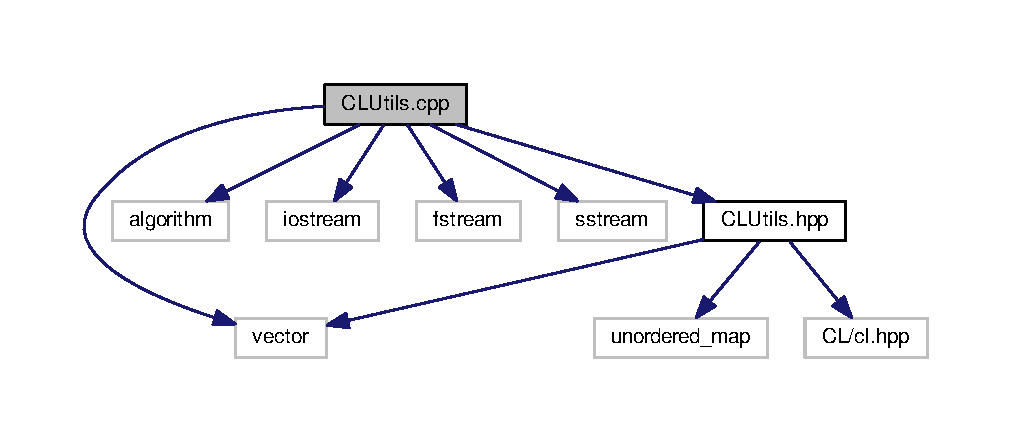
\includegraphics[width=350pt]{CLUtils_8cpp__incl}
\end{center}
\end{figure}
\subsection*{Namespaces}
\begin{DoxyCompactItemize}
\item 
 \hyperlink{namespaceclutils}{clutils}
\begin{DoxyCompactList}\small\item\em It brings together functionality common to all Open\+C\+L projects. \end{DoxyCompactList}\end{DoxyCompactItemize}
\subsection*{Functions}
\begin{DoxyCompactItemize}
\item 
const char $\ast$ \hyperlink{namespaceclutils_a8741b6850668dbbdb8a283122365c1d9}{clutils\+::get\+Open\+C\+L\+Error\+Code\+String} (int error\+Code)
\begin{DoxyCompactList}\small\item\em Returns the name of an error code. \end{DoxyCompactList}\item 
void \hyperlink{namespaceclutils_aade8becb266bc2e98a7b37f05001011e}{clutils\+::read\+Source} (const std\+::vector$<$ std\+::string $>$ \&kernel\+\_\+filenames, std\+::vector$<$ std\+::string $>$ \&source\+Codes)
\begin{DoxyCompactList}\small\item\em Reads in the contents from the requested files. \end{DoxyCompactList}\item 
void \hyperlink{namespaceclutils_a585a32b5c93ecbbf1f233b362f76e988}{clutils\+::split} (const std\+::string \&str, char delim, std\+::vector$<$ std\+::string $>$ \&names)
\begin{DoxyCompactList}\small\item\em Splits a string on the requested delimiter. \end{DoxyCompactList}\item 
std\+::pair$<$ const char $\ast$, size\+\_\+t $>$ \hyperlink{namespaceclutils_a485db8206a6181bbba6e1a110c0b9bb2}{clutils\+::make\+\_\+kernel\+\_\+pair} (const std\+::string \&kernel\+\_\+filename)
\begin{DoxyCompactList}\small\item\em Creates a pair of a char array (source code) and its size. \end{DoxyCompactList}\end{DoxyCompactItemize}


\subsection{Detailed Description}
Definitions of functions and methods for the C\+L\+Utils library. 

C\+L\+Utils offers utilities that help setup and manage an Open\+C\+L environment. \begin{DoxyAuthor}{Author}
Nick Lamprianidis 
\end{DoxyAuthor}
\begin{DoxyVersion}{Version}
0.\+1 
\end{DoxyVersion}
\begin{DoxyDate}{Date}
2014-\/2015 
\end{DoxyDate}
\begin{DoxyCopyright}{Copyright}
The M\+I\+T License (M\+I\+T) 
\end{DoxyCopyright}
\begin{DoxyParagraph}{}
Copyright (c) 2014 Nick Lamprianidis 
\end{DoxyParagraph}
\begin{DoxyParagraph}{}
Permission is hereby granted, free of charge, to any person obtaining a copy of this software and associated documentation files (the \char`\"{}\+Software\char`\"{}), to deal in the Software without restriction, including without limitation the rights to use, copy, modify, merge, publish, distribute, sublicense, and/or sell copies of the Software, and to permit persons to whom the Software is furnished to do so, subject to the following conditions\+: 
\end{DoxyParagraph}
\begin{DoxyParagraph}{}
The above copyright notice and this permission notice shall be included in all copies or substantial portions of the Software. 
\end{DoxyParagraph}
\begin{DoxyParagraph}{}
T\+H\+E S\+O\+F\+T\+W\+A\+R\+E I\+S P\+R\+O\+V\+I\+D\+E\+D \char`\"{}\+A\+S I\+S\char`\"{}, W\+I\+T\+H\+O\+U\+T W\+A\+R\+R\+A\+N\+T\+Y O\+F A\+N\+Y K\+I\+N\+D, E\+X\+P\+R\+E\+S\+S O\+R I\+M\+P\+L\+I\+E\+D, I\+N\+C\+L\+U\+D\+I\+N\+G B\+U\+T N\+O\+T L\+I\+M\+I\+T\+E\+D T\+O T\+H\+E W\+A\+R\+R\+A\+N\+T\+I\+E\+S O\+F M\+E\+R\+C\+H\+A\+N\+T\+A\+B\+I\+L\+I\+T\+Y, F\+I\+T\+N\+E\+S\+S F\+O\+R A P\+A\+R\+T\+I\+C\+U\+L\+A\+R P\+U\+R\+P\+O\+S\+E A\+N\+D N\+O\+N\+I\+N\+F\+R\+I\+N\+G\+E\+M\+E\+N\+T. I\+N N\+O E\+V\+E\+N\+T S\+H\+A\+L\+L T\+H\+E A\+U\+T\+H\+O\+R\+S O\+R C\+O\+P\+Y\+R\+I\+G\+H\+T H\+O\+L\+D\+E\+R\+S B\+E L\+I\+A\+B\+L\+E F\+O\+R A\+N\+Y C\+L\+A\+I\+M, D\+A\+M\+A\+G\+E\+S O\+R O\+T\+H\+E\+R L\+I\+A\+B\+I\+L\+I\+T\+Y, W\+H\+E\+T\+H\+E\+R I\+N A\+N A\+C\+T\+I\+O\+N O\+F C\+O\+N\+T\+R\+A\+C\+T, T\+O\+R\+T O\+R O\+T\+H\+E\+R\+W\+I\+S\+E, A\+R\+I\+S\+I\+N\+G F\+R\+O\+M, O\+U\+T O\+F O\+R I\+N C\+O\+N\+N\+E\+C\+T\+I\+O\+N W\+I\+T\+H T\+H\+E S\+O\+F\+T\+W\+A\+R\+E O\+R T\+H\+E U\+S\+E O\+R O\+T\+H\+E\+R D\+E\+A\+L\+I\+N\+G\+S I\+N T\+H\+E S\+O\+F\+T\+W\+A\+R\+E. 
\end{DoxyParagraph}

\hypertarget{CLUtils_8hpp}{}\section{C\+L\+Utils.\+hpp File Reference}
\label{CLUtils_8hpp}\index{C\+L\+Utils.\+hpp@{C\+L\+Utils.\+hpp}}


Declarations of objects, functions and classes for the C\+L\+Utils library.  


{\ttfamily \#include $<$vector$>$}\\*
{\ttfamily \#include $<$unordered\+\_\+map$>$}\\*
{\ttfamily \#include $<$C\+L/cl.\+hpp$>$}\\*
Include dependency graph for C\+L\+Utils.\+hpp\+:
\nopagebreak
\begin{figure}[H]
\begin{center}
\leavevmode
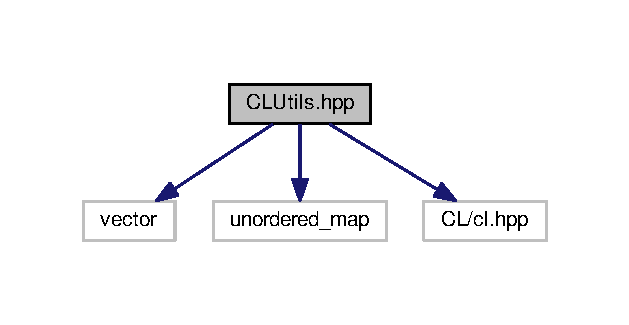
\includegraphics[width=302pt]{CLUtils_8hpp__incl}
\end{center}
\end{figure}
This graph shows which files directly or indirectly include this file\+:
\nopagebreak
\begin{figure}[H]
\begin{center}
\leavevmode
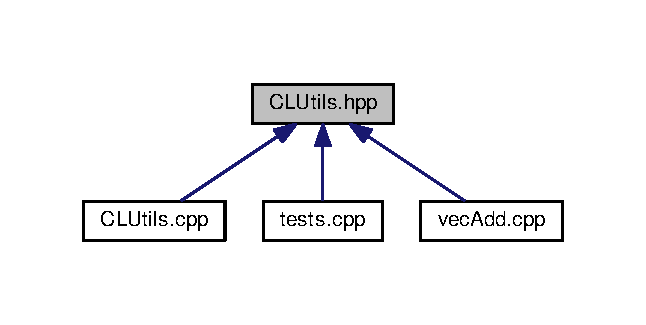
\includegraphics[width=310pt]{CLUtils_8hpp__dep__incl}
\end{center}
\end{figure}
\subsection*{Classes}
\begin{DoxyCompactItemize}
\item 
class \hyperlink{classclutils_1_1CLEnv}{clutils\+::\+C\+L\+Env}
\begin{DoxyCompactList}\small\item\em Sets up an Open\+C\+L environment. \end{DoxyCompactList}\end{DoxyCompactItemize}
\subsection*{Namespaces}
\begin{DoxyCompactItemize}
\item 
 \hyperlink{namespaceclutils}{clutils}
\begin{DoxyCompactList}\small\item\em It brings together functionality common to all Open\+C\+L projects. \end{DoxyCompactList}\end{DoxyCompactItemize}
\subsection*{Functions}
\begin{DoxyCompactItemize}
\item 
const char $\ast$ \hyperlink{namespaceclutils_a8741b6850668dbbdb8a283122365c1d9}{clutils\+::get\+Open\+C\+L\+Error\+Code\+String} (int error\+Code)
\begin{DoxyCompactList}\small\item\em Returns the name of an error code. \end{DoxyCompactList}\item 
void \hyperlink{namespaceclutils_aade8becb266bc2e98a7b37f05001011e}{clutils\+::read\+Source} (const std\+::vector$<$ std\+::string $>$ \&kernel\+\_\+filenames, std\+::vector$<$ std\+::string $>$ \&source\+Codes)
\begin{DoxyCompactList}\small\item\em Reads in the contents from the requested files. \end{DoxyCompactList}\item 
void \hyperlink{namespaceclutils_a585a32b5c93ecbbf1f233b362f76e988}{clutils\+::split} (const std\+::string \&str, char delim, std\+::vector$<$ std\+::string $>$ \&names)
\begin{DoxyCompactList}\small\item\em Splits a string on the requested delimiter. \end{DoxyCompactList}\item 
std\+::pair$<$ const char $\ast$, size\+\_\+t $>$ \hyperlink{namespaceclutils_a485db8206a6181bbba6e1a110c0b9bb2}{clutils\+::make\+\_\+kernel\+\_\+pair} (const std\+::string \&kernel\+\_\+filename)
\begin{DoxyCompactList}\small\item\em Creates a pair of a char array (source code) and its size. \end{DoxyCompactList}\end{DoxyCompactItemize}


\subsection{Detailed Description}
Declarations of objects, functions and classes for the C\+L\+Utils library. 

C\+L\+Utils offers utilities that help setup and manage an Open\+C\+L environment. \begin{DoxyAuthor}{Author}
Nick Lamprianidis 
\end{DoxyAuthor}
\begin{DoxyVersion}{Version}
0.\+1 
\end{DoxyVersion}
\begin{DoxyDate}{Date}
2014-\/2015 
\end{DoxyDate}
\begin{DoxyCopyright}{Copyright}
The M\+I\+T License (M\+I\+T) 
\end{DoxyCopyright}
\begin{DoxyParagraph}{}
Copyright (c) 2014 Nick Lamprianidis 
\end{DoxyParagraph}
\begin{DoxyParagraph}{}
Permission is hereby granted, free of charge, to any person obtaining a copy of this software and associated documentation files (the \char`\"{}\+Software\char`\"{}), to deal in the Software without restriction, including without limitation the rights to use, copy, modify, merge, publish, distribute, sublicense, and/or sell copies of the Software, and to permit persons to whom the Software is furnished to do so, subject to the following conditions\+: 
\end{DoxyParagraph}
\begin{DoxyParagraph}{}
The above copyright notice and this permission notice shall be included in all copies or substantial portions of the Software. 
\end{DoxyParagraph}
\begin{DoxyParagraph}{}
T\+H\+E S\+O\+F\+T\+W\+A\+R\+E I\+S P\+R\+O\+V\+I\+D\+E\+D \char`\"{}\+A\+S I\+S\char`\"{}, W\+I\+T\+H\+O\+U\+T W\+A\+R\+R\+A\+N\+T\+Y O\+F A\+N\+Y K\+I\+N\+D, E\+X\+P\+R\+E\+S\+S O\+R I\+M\+P\+L\+I\+E\+D, I\+N\+C\+L\+U\+D\+I\+N\+G B\+U\+T N\+O\+T L\+I\+M\+I\+T\+E\+D T\+O T\+H\+E W\+A\+R\+R\+A\+N\+T\+I\+E\+S O\+F M\+E\+R\+C\+H\+A\+N\+T\+A\+B\+I\+L\+I\+T\+Y, F\+I\+T\+N\+E\+S\+S F\+O\+R A P\+A\+R\+T\+I\+C\+U\+L\+A\+R P\+U\+R\+P\+O\+S\+E A\+N\+D N\+O\+N\+I\+N\+F\+R\+I\+N\+G\+E\+M\+E\+N\+T. I\+N N\+O E\+V\+E\+N\+T S\+H\+A\+L\+L T\+H\+E A\+U\+T\+H\+O\+R\+S O\+R C\+O\+P\+Y\+R\+I\+G\+H\+T H\+O\+L\+D\+E\+R\+S B\+E L\+I\+A\+B\+L\+E F\+O\+R A\+N\+Y C\+L\+A\+I\+M, D\+A\+M\+A\+G\+E\+S O\+R O\+T\+H\+E\+R L\+I\+A\+B\+I\+L\+I\+T\+Y, W\+H\+E\+T\+H\+E\+R I\+N A\+N A\+C\+T\+I\+O\+N O\+F C\+O\+N\+T\+R\+A\+C\+T, T\+O\+R\+T O\+R O\+T\+H\+E\+R\+W\+I\+S\+E, A\+R\+I\+S\+I\+N\+G F\+R\+O\+M, O\+U\+T O\+F O\+R I\+N C\+O\+N\+N\+E\+C\+T\+I\+O\+N W\+I\+T\+H T\+H\+E S\+O\+F\+T\+W\+A\+R\+E O\+R T\+H\+E U\+S\+E O\+R O\+T\+H\+E\+R D\+E\+A\+L\+I\+N\+G\+S I\+N T\+H\+E S\+O\+F\+T\+W\+A\+R\+E. 
\end{DoxyParagraph}

\hypertarget{kernels_8cl}{}\section{kernels.\+cl File Reference}
\label{kernels_8cl}\index{kernels.\+cl@{kernels.\+cl}}


It contains a kernel that performs a vector addition.  


\subsection*{Functions}
\begin{DoxyCompactItemize}
\item 
\+\_\+\+\_\+kernel void \hyperlink{kernels_8cl_a15fe8af998456b32910ce0c06f12a87e}{vec\+Add} (\+\_\+\+\_\+global int $\ast$A, \+\_\+\+\_\+global int $\ast$B, \+\_\+\+\_\+global int $\ast$C)
\begin{DoxyCompactList}\small\item\em It performs a vector addition. \end{DoxyCompactList}\end{DoxyCompactItemize}


\subsection{Detailed Description}
It contains a kernel that performs a vector addition. 

\begin{DoxyAuthor}{Author}
Nick Lamprianidis 
\end{DoxyAuthor}
\begin{DoxyVersion}{Version}
1.\+0 
\end{DoxyVersion}
\begin{DoxyDate}{Date}
2014-\/2015 
\end{DoxyDate}
\begin{DoxyCopyright}{Copyright}
The M\+I\+T License (M\+I\+T) 
\end{DoxyCopyright}
\begin{DoxyParagraph}{}
Copyright (c) 2014 Nick Lamprianidis 
\end{DoxyParagraph}
\begin{DoxyParagraph}{}
Permission is hereby granted, free of charge, to any person obtaining a copy of this software and associated documentation files (the \char`\"{}\+Software\char`\"{}), to deal in the Software without restriction, including without limitation the rights to use, copy, modify, merge, publish, distribute, sublicense, and/or sell copies of the Software, and to permit persons to whom the Software is furnished to do so, subject to the following conditions\+: 
\end{DoxyParagraph}
\begin{DoxyParagraph}{}
The above copyright notice and this permission notice shall be included in all copies or substantial portions of the Software. 
\end{DoxyParagraph}
\begin{DoxyParagraph}{}
T\+H\+E S\+O\+F\+T\+W\+A\+R\+E I\+S P\+R\+O\+V\+I\+D\+E\+D \char`\"{}\+A\+S I\+S\char`\"{}, W\+I\+T\+H\+O\+U\+T W\+A\+R\+R\+A\+N\+T\+Y O\+F A\+N\+Y K\+I\+N\+D, E\+X\+P\+R\+E\+S\+S O\+R I\+M\+P\+L\+I\+E\+D, I\+N\+C\+L\+U\+D\+I\+N\+G B\+U\+T N\+O\+T L\+I\+M\+I\+T\+E\+D T\+O T\+H\+E W\+A\+R\+R\+A\+N\+T\+I\+E\+S O\+F M\+E\+R\+C\+H\+A\+N\+T\+A\+B\+I\+L\+I\+T\+Y, F\+I\+T\+N\+E\+S\+S F\+O\+R A P\+A\+R\+T\+I\+C\+U\+L\+A\+R P\+U\+R\+P\+O\+S\+E A\+N\+D N\+O\+N\+I\+N\+F\+R\+I\+N\+G\+E\+M\+E\+N\+T. I\+N N\+O E\+V\+E\+N\+T S\+H\+A\+L\+L T\+H\+E A\+U\+T\+H\+O\+R\+S O\+R C\+O\+P\+Y\+R\+I\+G\+H\+T H\+O\+L\+D\+E\+R\+S B\+E L\+I\+A\+B\+L\+E F\+O\+R A\+N\+Y C\+L\+A\+I\+M, D\+A\+M\+A\+G\+E\+S O\+R O\+T\+H\+E\+R L\+I\+A\+B\+I\+L\+I\+T\+Y, W\+H\+E\+T\+H\+E\+R I\+N A\+N A\+C\+T\+I\+O\+N O\+F C\+O\+N\+T\+R\+A\+C\+T, T\+O\+R\+T O\+R O\+T\+H\+E\+R\+W\+I\+S\+E, A\+R\+I\+S\+I\+N\+G F\+R\+O\+M, O\+U\+T O\+F O\+R I\+N C\+O\+N\+N\+E\+C\+T\+I\+O\+N W\+I\+T\+H T\+H\+E S\+O\+F\+T\+W\+A\+R\+E O\+R T\+H\+E U\+S\+E O\+R O\+T\+H\+E\+R D\+E\+A\+L\+I\+N\+G\+S I\+N T\+H\+E S\+O\+F\+T\+W\+A\+R\+E. 
\end{DoxyParagraph}


\subsection{Function Documentation}
\hypertarget{kernels_8cl_a15fe8af998456b32910ce0c06f12a87e}{}\index{kernels.\+cl@{kernels.\+cl}!vec\+Add@{vec\+Add}}
\index{vec\+Add@{vec\+Add}!kernels.\+cl@{kernels.\+cl}}
\subsubsection[{vec\+Add}]{\setlength{\rightskip}{0pt plus 5cm}\+\_\+\+\_\+kernel void {\bf vec\+Add} (
\begin{DoxyParamCaption}
\item[{\+\_\+\+\_\+global int $\ast$}]{A, }
\item[{\+\_\+\+\_\+global int $\ast$}]{B, }
\item[{\+\_\+\+\_\+global int $\ast$}]{C}
\end{DoxyParamCaption}
)}\label{kernels_8cl_a15fe8af998456b32910ce0c06f12a87e}


It performs a vector addition. 


\begin{DoxyParams}[1]{Parameters}
\mbox{\tt in}  & {\em A} & first operand (buffer) to the vector addition. \\
\hline
\mbox{\tt in}  & {\em B} & second operand (buffer) to the vector addition. \\
\hline
\mbox{\tt out}  & {\em C} & holds the result (buffer) of the vector addition. \\
\hline
\end{DoxyParams}

\hypertarget{kernels2_8cl}{}\section{kernels2.\+cl File Reference}
\label{kernels2_8cl}\index{kernels2.\+cl@{kernels2.\+cl}}


It contains a kernel for buffer initialization.  


\subsection*{Functions}
\begin{DoxyCompactItemize}
\item 
\+\_\+\+\_\+kernel void \hyperlink{kernels2_8cl_a6492bce4361004090b61f519f83482b4}{init\+Rand} (\+\_\+\+\_\+global int $\ast$A)
\begin{DoxyCompactList}\small\item\em It initializes a buffer. \end{DoxyCompactList}\end{DoxyCompactItemize}


\subsection{Detailed Description}
It contains a kernel for buffer initialization. 

\begin{DoxyAuthor}{Author}
Nick Lamprianidis 
\end{DoxyAuthor}
\begin{DoxyVersion}{Version}
1.\+0 
\end{DoxyVersion}
\begin{DoxyDate}{Date}
2014-\/2015 
\end{DoxyDate}
\begin{DoxyCopyright}{Copyright}
The M\+I\+T License (M\+I\+T) 
\end{DoxyCopyright}
\begin{DoxyParagraph}{}
Copyright (c) 2014 Nick Lamprianidis 
\end{DoxyParagraph}
\begin{DoxyParagraph}{}
Permission is hereby granted, free of charge, to any person obtaining a copy of this software and associated documentation files (the \char`\"{}\+Software\char`\"{}), to deal in the Software without restriction, including without limitation the rights to use, copy, modify, merge, publish, distribute, sublicense, and/or sell copies of the Software, and to permit persons to whom the Software is furnished to do so, subject to the following conditions\+: 
\end{DoxyParagraph}
\begin{DoxyParagraph}{}
The above copyright notice and this permission notice shall be included in all copies or substantial portions of the Software. 
\end{DoxyParagraph}
\begin{DoxyParagraph}{}
T\+H\+E S\+O\+F\+T\+W\+A\+R\+E I\+S P\+R\+O\+V\+I\+D\+E\+D \char`\"{}\+A\+S I\+S\char`\"{}, W\+I\+T\+H\+O\+U\+T W\+A\+R\+R\+A\+N\+T\+Y O\+F A\+N\+Y K\+I\+N\+D, E\+X\+P\+R\+E\+S\+S O\+R I\+M\+P\+L\+I\+E\+D, I\+N\+C\+L\+U\+D\+I\+N\+G B\+U\+T N\+O\+T L\+I\+M\+I\+T\+E\+D T\+O T\+H\+E W\+A\+R\+R\+A\+N\+T\+I\+E\+S O\+F M\+E\+R\+C\+H\+A\+N\+T\+A\+B\+I\+L\+I\+T\+Y, F\+I\+T\+N\+E\+S\+S F\+O\+R A P\+A\+R\+T\+I\+C\+U\+L\+A\+R P\+U\+R\+P\+O\+S\+E A\+N\+D N\+O\+N\+I\+N\+F\+R\+I\+N\+G\+E\+M\+E\+N\+T. I\+N N\+O E\+V\+E\+N\+T S\+H\+A\+L\+L T\+H\+E A\+U\+T\+H\+O\+R\+S O\+R C\+O\+P\+Y\+R\+I\+G\+H\+T H\+O\+L\+D\+E\+R\+S B\+E L\+I\+A\+B\+L\+E F\+O\+R A\+N\+Y C\+L\+A\+I\+M, D\+A\+M\+A\+G\+E\+S O\+R O\+T\+H\+E\+R L\+I\+A\+B\+I\+L\+I\+T\+Y, W\+H\+E\+T\+H\+E\+R I\+N A\+N A\+C\+T\+I\+O\+N O\+F C\+O\+N\+T\+R\+A\+C\+T, T\+O\+R\+T O\+R O\+T\+H\+E\+R\+W\+I\+S\+E, A\+R\+I\+S\+I\+N\+G F\+R\+O\+M, O\+U\+T O\+F O\+R I\+N C\+O\+N\+N\+E\+C\+T\+I\+O\+N W\+I\+T\+H T\+H\+E S\+O\+F\+T\+W\+A\+R\+E O\+R T\+H\+E U\+S\+E O\+R O\+T\+H\+E\+R D\+E\+A\+L\+I\+N\+G\+S I\+N T\+H\+E S\+O\+F\+T\+W\+A\+R\+E. 
\end{DoxyParagraph}


\subsection{Function Documentation}
\hypertarget{kernels2_8cl_a6492bce4361004090b61f519f83482b4}{}\index{kernels2.\+cl@{kernels2.\+cl}!init\+Rand@{init\+Rand}}
\index{init\+Rand@{init\+Rand}!kernels2.\+cl@{kernels2.\+cl}}
\subsubsection[{init\+Rand}]{\setlength{\rightskip}{0pt plus 5cm}\+\_\+\+\_\+kernel void init\+Rand (
\begin{DoxyParamCaption}
\item[{\+\_\+\+\_\+global int $\ast$}]{A}
\end{DoxyParamCaption}
)}\label{kernels2_8cl_a6492bce4361004090b61f519f83482b4}


It initializes a buffer. 

\begin{DoxyNote}{Note}
The kernel expects a define directive (I\+N\+I\+T\+\_\+\+N\+U\+M). This is provided as a command line argument. 
\end{DoxyNote}

\begin{DoxyParams}[1]{Parameters}
\mbox{\tt in}  & {\em A} & a buffer to initialize. \\
\hline
\end{DoxyParams}

\hypertarget{tests_8cpp}{}\section{tests.\+cpp File Reference}
\label{tests_8cpp}\index{tests.\+cpp@{tests.\+cpp}}


Google Test Unit Tests.  


{\ttfamily \#include $<$gtest/gtest.\+h$>$}\\*
{\ttfamily \#include $<$iostream$>$}\\*
{\ttfamily \#include $<$vector$>$}\\*
{\ttfamily \#include $<$chrono$>$}\\*
{\ttfamily \#include $<$random$>$}\\*
{\ttfamily \#include $<$C\+L\+Utils.\+hpp$>$}\\*
Include dependency graph for tests.\+cpp\+:
\nopagebreak
\begin{figure}[H]
\begin{center}
\leavevmode
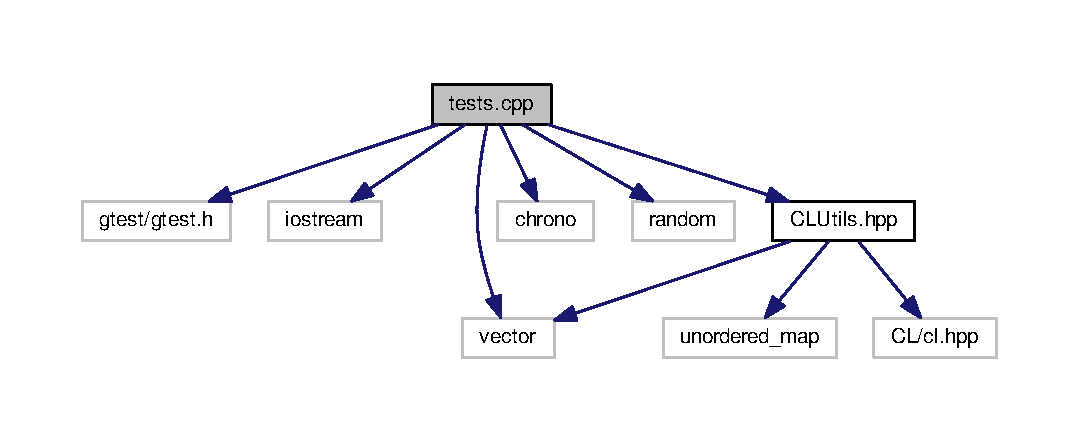
\includegraphics[width=350pt]{tests_8cpp__incl}
\end{center}
\end{figure}
\subsection*{Functions}
\begin{DoxyCompactItemize}
\item 
\hypertarget{tests_8cpp_a7739f9a14ee87e088af1af3ba2bdada3}{}std\+::default\+\_\+random\+\_\+engine {\bfseries generator} (seed)\label{tests_8cpp_a7739f9a14ee87e088af1af3ba2bdada3}

\item 
\hypertarget{tests_8cpp_a011ffc8e39fc421d91989cde3df3e77e}{}std\+::uniform\+\_\+int\+\_\+distribution$<$ int $>$ {\bfseries distribution} (1, 32)\label{tests_8cpp_a011ffc8e39fc421d91989cde3df3e77e}

\item 
\hypertarget{tests_8cpp_ae77c6fe2fd10afe373583deb35f5bfe8}{}\hyperlink{tests_8cpp_ae77c6fe2fd10afe373583deb35f5bfe8}{T\+E\+S\+T} (C\+L\+Env, Basic\+Functionality)\label{tests_8cpp_ae77c6fe2fd10afe373583deb35f5bfe8}

\begin{DoxyCompactList}\small\item\em Performs a buffer initialization under default environment. \end{DoxyCompactList}\item 
\hypertarget{tests_8cpp_ac49a60d8ae82d0c0c0c1ae8329ca35f0}{}\hyperlink{tests_8cpp_ac49a60d8ae82d0c0c0c1ae8329ca35f0}{T\+E\+S\+T} (C\+L\+Env, Add\+More\+C\+L\+Objects)\label{tests_8cpp_ac49a60d8ae82d0c0c0c1ae8329ca35f0}

\begin{DoxyCompactList}\small\item\em Performs a buffer initializations and a vector addition under user created environment. \end{DoxyCompactList}\item 
\hypertarget{tests_8cpp_a3c04138a5bfe5d72780bb7e82a18e627}{}int {\bfseries main} (int argc, char $\ast$$\ast$argv)\label{tests_8cpp_a3c04138a5bfe5d72780bb7e82a18e627}

\end{DoxyCompactItemize}
\subsection*{Variables}
\begin{DoxyCompactItemize}
\item 
\hypertarget{tests_8cpp_a0d541b084e401409a4486b7ec3d24381}{}const std\+::string {\bfseries kernel\+\_\+filename} \{ \char`\"{}kernels/kernels.\+cl\char`\"{} \}\label{tests_8cpp_a0d541b084e401409a4486b7ec3d24381}

\item 
\hypertarget{tests_8cpp_a7c2b91c223865d7e861ab57e7476ea7b}{}const std\+::string {\bfseries kernel\+\_\+filename2} \{ \char`\"{}kernels/kernels2.\+cl\char`\"{} \}\label{tests_8cpp_a7c2b91c223865d7e861ab57e7476ea7b}

\item 
\hypertarget{tests_8cpp_a76b58816d636a123eea7f876077cae64}{}const std\+::vector$<$ std\+::string $>$ {\bfseries kernel\+\_\+filenames} \{ kernel\+\_\+filename, kernel\+\_\+filename2 \}\label{tests_8cpp_a76b58816d636a123eea7f876077cae64}

\item 
\hypertarget{tests_8cpp_a08668fde34d014a7ab1191a1ccf501e3}{}const int {\bfseries n\+\_\+elements} = 1$<$$<$12\label{tests_8cpp_a08668fde34d014a7ab1191a1ccf501e3}

\item 
\hypertarget{tests_8cpp_abff8079048cc60fc6a425dcf1c41254a}{}auto {\bfseries seed} = std\+::chrono\+::system\+\_\+clock\+::now ().time\+\_\+since\+\_\+epoch ().count ()\label{tests_8cpp_abff8079048cc60fc6a425dcf1c41254a}

\item 
auto \hyperlink{tests_8cpp_aa156ca8a20d1ac9a126f31baed86c672}{r\+Num} = std\+::bind (distribution, generator)
\end{DoxyCompactItemize}


\subsection{Detailed Description}
Google Test Unit Tests. 

\begin{DoxyAuthor}{Author}
Nick Lamprianidis 
\end{DoxyAuthor}
\begin{DoxyVersion}{Version}
0.\+1 
\end{DoxyVersion}
\begin{DoxyDate}{Date}
2014-\/2015 
\end{DoxyDate}
\begin{DoxyCopyright}{Copyright}
The M\+I\+T License (M\+I\+T) 
\end{DoxyCopyright}
\begin{DoxyParagraph}{}
Copyright (c) 2014 Nick Lamprianidis 
\end{DoxyParagraph}
\begin{DoxyParagraph}{}
Permission is hereby granted, free of charge, to any person obtaining a copy of this software and associated documentation files (the \char`\"{}\+Software\char`\"{}), to deal in the Software without restriction, including without limitation the rights to use, copy, modify, merge, publish, distribute, sublicense, and/or sell copies of the Software, and to permit persons to whom the Software is furnished to do so, subject to the following conditions\+: 
\end{DoxyParagraph}
\begin{DoxyParagraph}{}
The above copyright notice and this permission notice shall be included in all copies or substantial portions of the Software. 
\end{DoxyParagraph}
\begin{DoxyParagraph}{}
T\+H\+E S\+O\+F\+T\+W\+A\+R\+E I\+S P\+R\+O\+V\+I\+D\+E\+D \char`\"{}\+A\+S I\+S\char`\"{}, W\+I\+T\+H\+O\+U\+T W\+A\+R\+R\+A\+N\+T\+Y O\+F A\+N\+Y K\+I\+N\+D, E\+X\+P\+R\+E\+S\+S O\+R I\+M\+P\+L\+I\+E\+D, I\+N\+C\+L\+U\+D\+I\+N\+G B\+U\+T N\+O\+T L\+I\+M\+I\+T\+E\+D T\+O T\+H\+E W\+A\+R\+R\+A\+N\+T\+I\+E\+S O\+F M\+E\+R\+C\+H\+A\+N\+T\+A\+B\+I\+L\+I\+T\+Y, F\+I\+T\+N\+E\+S\+S F\+O\+R A P\+A\+R\+T\+I\+C\+U\+L\+A\+R P\+U\+R\+P\+O\+S\+E A\+N\+D N\+O\+N\+I\+N\+F\+R\+I\+N\+G\+E\+M\+E\+N\+T. I\+N N\+O E\+V\+E\+N\+T S\+H\+A\+L\+L T\+H\+E A\+U\+T\+H\+O\+R\+S O\+R C\+O\+P\+Y\+R\+I\+G\+H\+T H\+O\+L\+D\+E\+R\+S B\+E L\+I\+A\+B\+L\+E F\+O\+R A\+N\+Y C\+L\+A\+I\+M, D\+A\+M\+A\+G\+E\+S O\+R O\+T\+H\+E\+R L\+I\+A\+B\+I\+L\+I\+T\+Y, W\+H\+E\+T\+H\+E\+R I\+N A\+N A\+C\+T\+I\+O\+N O\+F C\+O\+N\+T\+R\+A\+C\+T, T\+O\+R\+T O\+R O\+T\+H\+E\+R\+W\+I\+S\+E, A\+R\+I\+S\+I\+N\+G F\+R\+O\+M, O\+U\+T O\+F O\+R I\+N C\+O\+N\+N\+E\+C\+T\+I\+O\+N W\+I\+T\+H T\+H\+E S\+O\+F\+T\+W\+A\+R\+E O\+R T\+H\+E U\+S\+E O\+R O\+T\+H\+E\+R D\+E\+A\+L\+I\+N\+G\+S I\+N T\+H\+E S\+O\+F\+T\+W\+A\+R\+E. 
\end{DoxyParagraph}


\subsection{Variable Documentation}
\hypertarget{tests_8cpp_aa156ca8a20d1ac9a126f31baed86c672}{}\index{tests.\+cpp@{tests.\+cpp}!r\+Num@{r\+Num}}
\index{r\+Num@{r\+Num}!tests.\+cpp@{tests.\+cpp}}
\subsubsection[{r\+Num}]{\setlength{\rightskip}{0pt plus 5cm}auto r\+Num = std\+::bind (distribution, generator)}\label{tests_8cpp_aa156ca8a20d1ac9a126f31baed86c672}
Produces a random integer with which device buffers will be initialized 
\hypertarget{vecAdd_8cpp}{}\section{vec\+Add.\+cpp File Reference}
\label{vecAdd_8cpp}\index{vec\+Add.\+cpp@{vec\+Add.\+cpp}}


An example showcasing the use of the C\+L\+Utils library. The executed kernel performs a vector addition.  


{\ttfamily \#include $<$iostream$>$}\\*
{\ttfamily \#include $<$vector$>$}\\*
{\ttfamily \#include $<$C\+L/cl.\+hpp$>$}\\*
{\ttfamily \#include $<$C\+L\+Utils.\+hpp$>$}\\*
Include dependency graph for vec\+Add.\+cpp\+:
\nopagebreak
\begin{figure}[H]
\begin{center}
\leavevmode
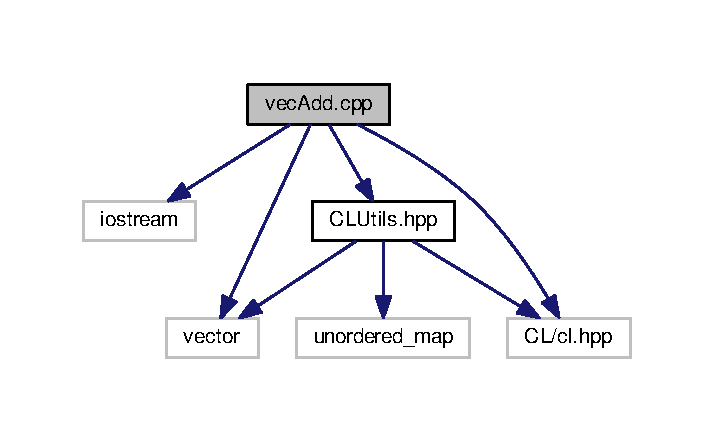
\includegraphics[width=342pt]{vecAdd_8cpp__incl}
\end{center}
\end{figure}
\subsection*{Classes}
\begin{DoxyCompactItemize}
\item 
class \hyperlink{classvecAdd}{vec\+Add}
\begin{DoxyCompactList}\small\item\em Creates an Open\+C\+L environment, and then performs a vector addition on the G\+P\+U. \end{DoxyCompactList}\end{DoxyCompactItemize}
\subsection*{Functions}
\begin{DoxyCompactItemize}
\item 
\hypertarget{vecAdd_8cpp_ae66f6b31b5ad750f1fe042a706a4e3d4}{}int {\bfseries main} ()\label{vecAdd_8cpp_ae66f6b31b5ad750f1fe042a706a4e3d4}

\end{DoxyCompactItemize}
\subsection*{Variables}
\begin{DoxyCompactItemize}
\item 
\hypertarget{vecAdd_8cpp_a0d541b084e401409a4486b7ec3d24381}{}const std\+::string {\bfseries kernel\+\_\+filename} \{ \char`\"{}kernels/kernels.\+cl\char`\"{} \}\label{vecAdd_8cpp_a0d541b084e401409a4486b7ec3d24381}

\item 
\hypertarget{vecAdd_8cpp_a08668fde34d014a7ab1191a1ccf501e3}{}const int {\bfseries n\+\_\+elements} = 1$<$$<$24\label{vecAdd_8cpp_a08668fde34d014a7ab1191a1ccf501e3}

\end{DoxyCompactItemize}


\subsection{Detailed Description}
An example showcasing the use of the C\+L\+Utils library. The executed kernel performs a vector addition. 

\begin{DoxyAuthor}{Author}
Nick Lamprianidis 
\end{DoxyAuthor}
\begin{DoxyVersion}{Version}
0.\+1 
\end{DoxyVersion}
\begin{DoxyDate}{Date}
2014-\/2015 
\end{DoxyDate}
\begin{DoxyCopyright}{Copyright}
The M\+I\+T License (M\+I\+T) 
\end{DoxyCopyright}
\begin{DoxyParagraph}{}
Copyright (c) 2014 Nick Lamprianidis 
\end{DoxyParagraph}
\begin{DoxyParagraph}{}
Permission is hereby granted, free of charge, to any person obtaining a copy of this software and associated documentation files (the \char`\"{}\+Software\char`\"{}), to deal in the Software without restriction, including without limitation the rights to use, copy, modify, merge, publish, distribute, sublicense, and/or sell copies of the Software, and to permit persons to whom the Software is furnished to do so, subject to the following conditions\+: 
\end{DoxyParagraph}
\begin{DoxyParagraph}{}
The above copyright notice and this permission notice shall be included in all copies or substantial portions of the Software. 
\end{DoxyParagraph}
\begin{DoxyParagraph}{}
T\+H\+E S\+O\+F\+T\+W\+A\+R\+E I\+S P\+R\+O\+V\+I\+D\+E\+D \char`\"{}\+A\+S I\+S\char`\"{}, W\+I\+T\+H\+O\+U\+T W\+A\+R\+R\+A\+N\+T\+Y O\+F A\+N\+Y K\+I\+N\+D, E\+X\+P\+R\+E\+S\+S O\+R I\+M\+P\+L\+I\+E\+D, I\+N\+C\+L\+U\+D\+I\+N\+G B\+U\+T N\+O\+T L\+I\+M\+I\+T\+E\+D T\+O T\+H\+E W\+A\+R\+R\+A\+N\+T\+I\+E\+S O\+F M\+E\+R\+C\+H\+A\+N\+T\+A\+B\+I\+L\+I\+T\+Y, F\+I\+T\+N\+E\+S\+S F\+O\+R A P\+A\+R\+T\+I\+C\+U\+L\+A\+R P\+U\+R\+P\+O\+S\+E A\+N\+D N\+O\+N\+I\+N\+F\+R\+I\+N\+G\+E\+M\+E\+N\+T. I\+N N\+O E\+V\+E\+N\+T S\+H\+A\+L\+L T\+H\+E A\+U\+T\+H\+O\+R\+S O\+R C\+O\+P\+Y\+R\+I\+G\+H\+T H\+O\+L\+D\+E\+R\+S B\+E L\+I\+A\+B\+L\+E F\+O\+R A\+N\+Y C\+L\+A\+I\+M, D\+A\+M\+A\+G\+E\+S O\+R O\+T\+H\+E\+R L\+I\+A\+B\+I\+L\+I\+T\+Y, W\+H\+E\+T\+H\+E\+R I\+N A\+N A\+C\+T\+I\+O\+N O\+F C\+O\+N\+T\+R\+A\+C\+T, T\+O\+R\+T O\+R O\+T\+H\+E\+R\+W\+I\+S\+E, A\+R\+I\+S\+I\+N\+G F\+R\+O\+M, O\+U\+T O\+F O\+R I\+N C\+O\+N\+N\+E\+C\+T\+I\+O\+N W\+I\+T\+H T\+H\+E S\+O\+F\+T\+W\+A\+R\+E O\+R T\+H\+E U\+S\+E O\+R O\+T\+H\+E\+R D\+E\+A\+L\+I\+N\+G\+S I\+N T\+H\+E S\+O\+F\+T\+W\+A\+R\+E. 
\end{DoxyParagraph}

%--- End generated contents ---

% Index
\backmatter
\newpage
\phantomsection
\clearemptydoublepage
\addcontentsline{toc}{chapter}{Index}
\printindex

\end{document}
